\documentclass[11pt]{scrartcl}
\usepackage[T1]{fontenc}
\usepackage[a4paper, left=3cm, right=2cm, top=2cm, bottom=2cm]{geometry}
\usepackage[activate]{pdfcprot}
\usepackage[ngerman]{babel}
\usepackage[parfill]{parskip}
\usepackage[utf8]{inputenc}
\usepackage{kurier}
\usepackage{amsmath}
\usepackage{amssymb}
\usepackage{xcolor}
\usepackage{epstopdf}
\usepackage{txfonts}
\usepackage{fancyhdr}
\usepackage{graphicx}
\usepackage{prettyref}
\usepackage{hyperref}
\usepackage{eurosym}
\usepackage{setspace}
\usepackage{units}
\usepackage{eso-pic,graphicx}
\usepackage{icomma}
\usepackage{pdfpages}

\definecolor{darkblue}{rgb}{0,0,.5}
\hypersetup{pdftex=true, colorlinks=true, breaklinks=false, linkcolor=black, menucolor=black, pagecolor=black, urlcolor=darkblue}



\setlength{\columnsep}{2cm}


\newcommand{\arcsinh}{\mathrm{arcsinh}}
\newcommand{\asinh}{\mathrm{arcsinh}}
\newcommand{\ergebnis}{\textcolor{red}{\mathrm{Ergebnis}}}
\newcommand{\fehlt}{\textcolor{red}{Hier fehlen noch Inhalte.}}
\newcommand{\betanotice}{\textcolor{red}{Diese Aufgaben sind noch nicht in der Übung kontrolliert worden. Es sind lediglich meine Überlegungen und Lösungsansätze zu den Aufgaben. Es können Fehler enthalten sein!!! Das Dokument wird fortwährend aktualisiert und erst wenn das \textcolor{black}{beta} aus dem Dateinamen verschwindet ist es endgültig.}}
\newcommand{\half}{\frac{1}{2}}
\renewcommand{\d}{\, \mathrm d}
\newcommand{\punkte}{\textcolor{white}{xxxxx}}
\newcommand{\p}{\, \partial}
\newcommand{\dd}[1]{\item[#1] \hfill \\}

\renewcommand{\familydefault}{\sfdefault}
\renewcommand\thesection{}
\renewcommand\thesubsection{}
\renewcommand\thesubsubsection{}


\newcommand{\themodul}{Optische Technologie}
\newcommand{\thetutor}{Prof. Rateike}
\newcommand{\theuebung}{Übung 2}

\pagestyle{fancy}
\fancyhead[L]{\footnotesize{C. Hansen}}
\chead{\thepage}
\rhead{}
\lfoot{}
\cfoot{}
\rfoot{}

\title{\themodul{}, \theuebung{}, \thetutor}


\author{Christoph Hansen \\ {\small \href{mailto:chris@university-material.de}{chris@university-material.de}} }

\date{}


\begin{document}

\maketitle

Dieser Text ist unter dieser \href{http://creativecommons.org/licenses/by-nc-sa/4.0/}{Creative Commons} Lizenz veröffentlicht.

\textcolor{red}{Ich erhebe keinen Anspruch auf Vollständigkeit oder Richtigkeit. Falls ihr Fehler findet oder etwas fehlt, dann meldet euch bitte über den Emailkontakt.}

\tableofcontents


\newpage



\section{Aufgabe 1}


\subsection*{a)}

Wir müssen uns klarmachen, das die Bildweite hier $b = -S_0$ ist:

\begin{align*}
\frac{1}{f} &= \frac{1}{g} + \frac{1}{b} = \frac{1}{g} - \frac{1}{S_0} \\
V &= - \frac{b}{g} = - \frac{-S_0}{g} = S_0 \cdot \left( \frac{1}{f} + \frac{1}{S_0} \right) = \frac{S_0}{f} + 1
\end{align*}


\subsection*{b)}

Dioptrin ist einfach der Kehrwert der Brennweite, also können wir folgendermaßen rechnen:

\begin{align*}
f &= \frac{1}{D} = \frac{1}{20} = \unit[5]{cm} \\
V &= \frac{S_0}{f} + 1 = \frac{30}{5} + 1 = 7
\end{align*}


\section{Aufgabe 2}


Wir legen die Größen fest:

\begin{align*}
G = \unit[2]{m} \qquad g &= \unit[50]{m} \qquad B = \unit[36]{mm} \\
\hfill \\
\left| \frac{B}{G} \right| &= \frac{b}{g} \\
\Leftrightarrow b &= g \cdot \frac{B}{G} = 50 \cdot \frac{36 \cdot 10^{-3}}{2} = \unit[0,9]{m} \\
\hfill \\
f &= \frac{1}{\frac{1}{50} + \frac{1}{0,9}} = \unit[0,88]{m}
\end{align*}


\newpage

\section{Aufgabe 3}

Wir haben die Situation auf dem Bild:

\begin{figure}[h]
	\centering
	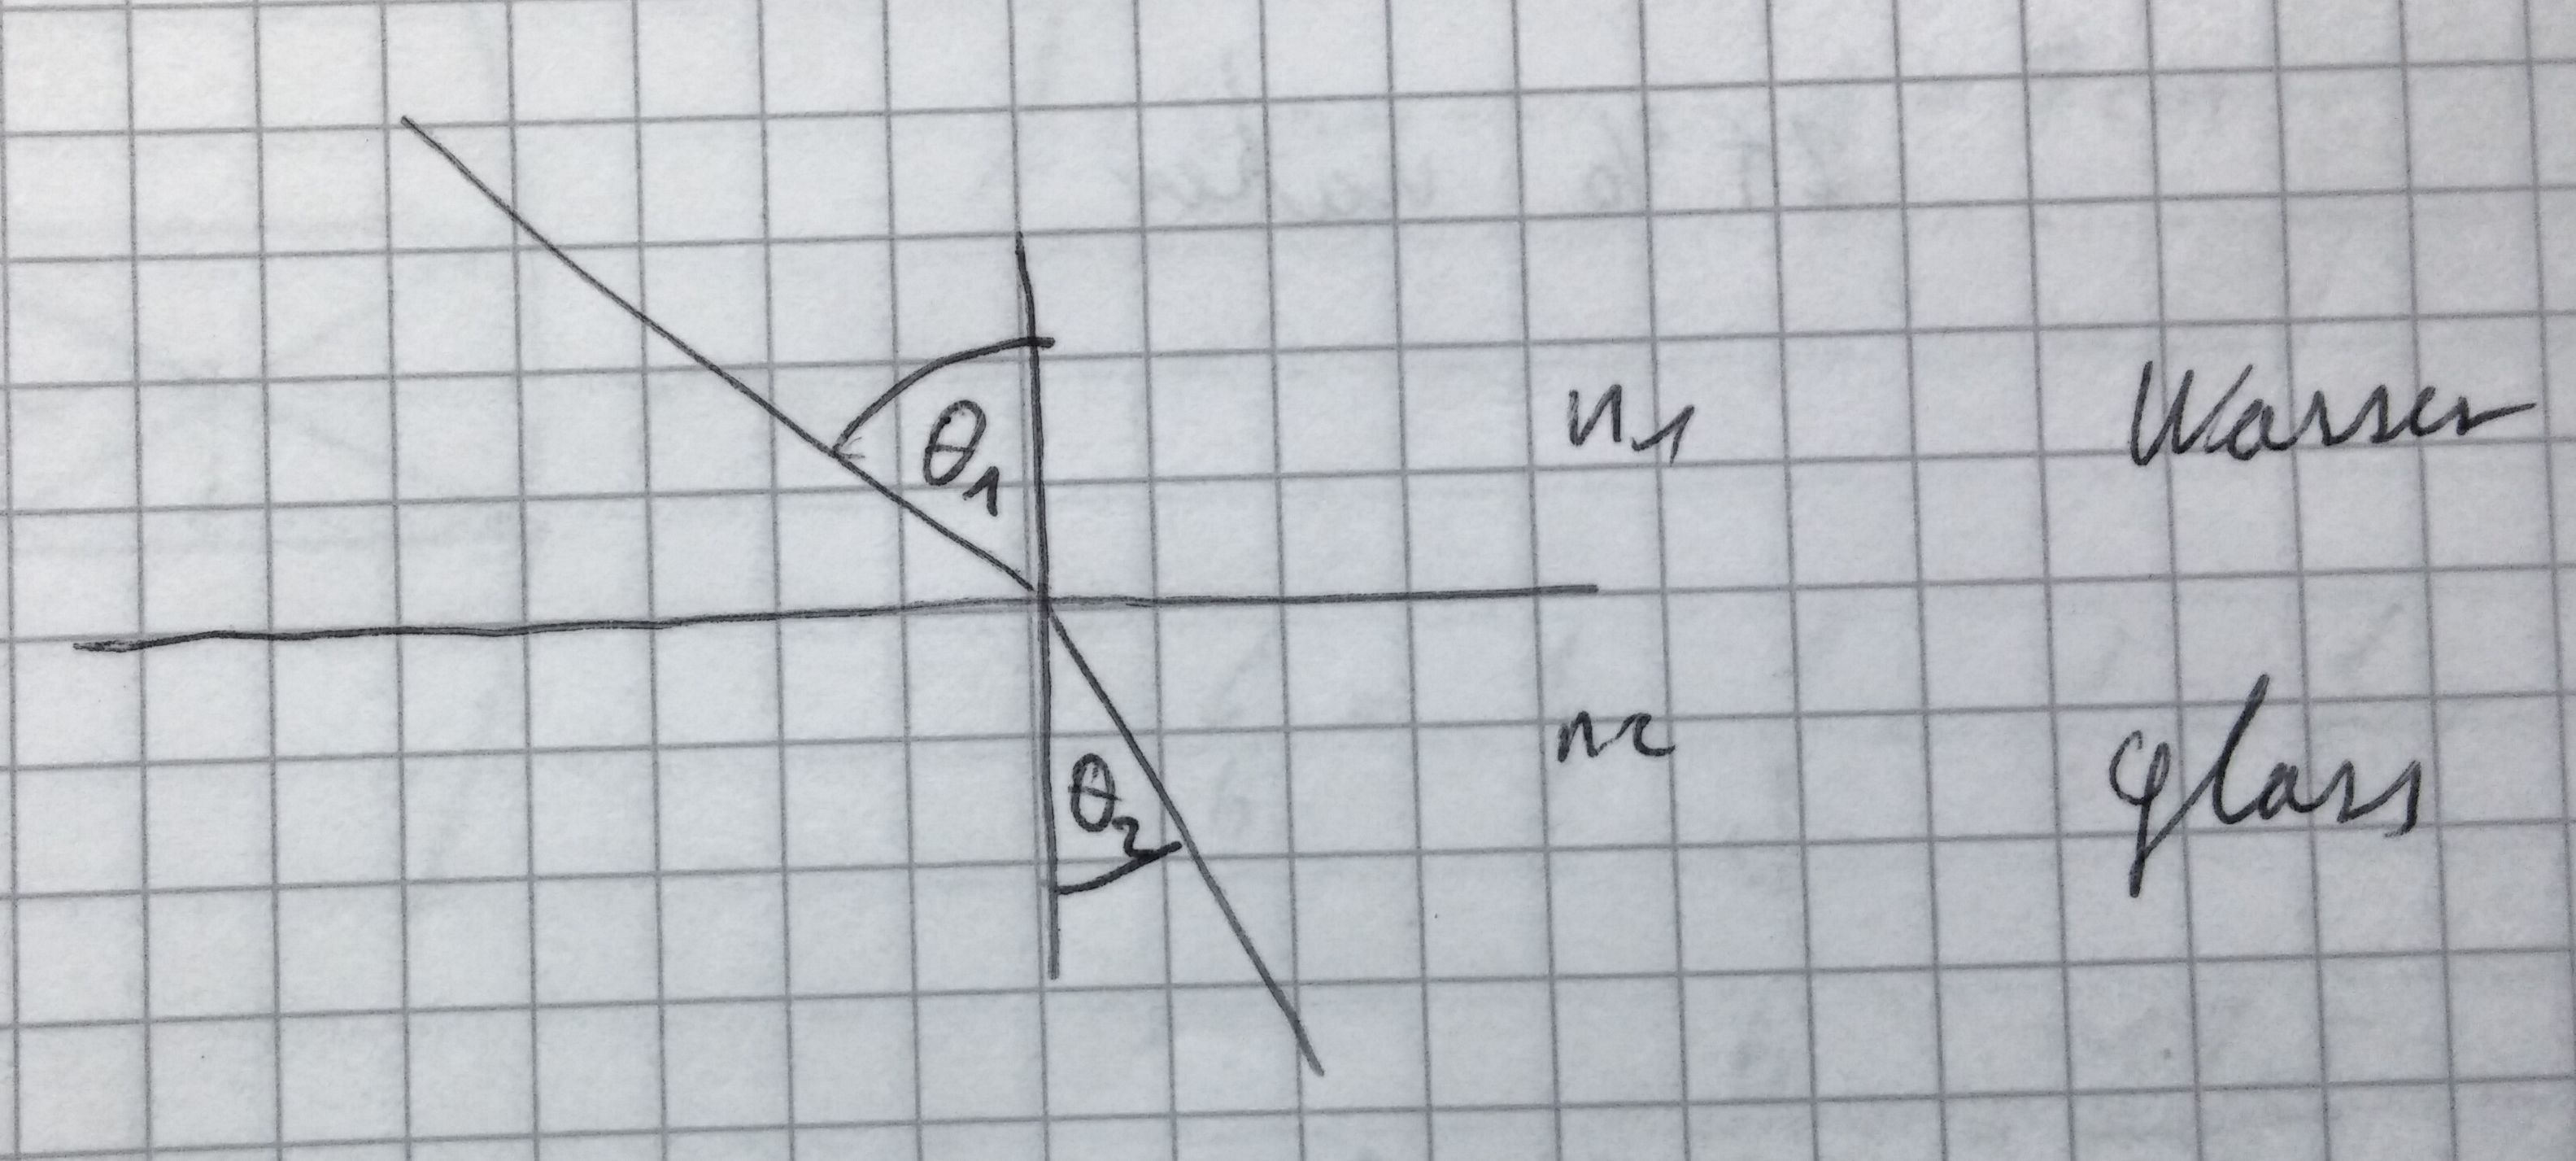
\includegraphics[scale=0.15]{A3_1.jpg}
\end{figure}


\begin{align*}
g &= \unit[23]{cm} \qquad b = \unit[-48]{cm} \\
\hfill \\
f &= \frac{1}{\frac{1}{23} - \frac{1}{48}} = \unit[0,44]{m} \\
D &= \frac{1}{f} = \frac{1}{0,44} = \unit[2,27]{dpt}
\end{align*}


\section{Aufgabe 4}

Wir wissen, das gilt:

\begin{align*}
\frac{f_{Ob}}{f_{Ok}} &= 7 \\
\Leftrightarrow f_{Ob} &= 7 \cdot f_{Ok} \\
\hfill \\
f_{Ob} + f_{Ok} &= 32 = 7 \cdot f_{Ok} + f_{Ok} \\
\Rightarrow f_{Ok} &= \unit[4]{cm} \qquad f_{Ob} = \unit[28]{cm}
\end{align*}

\newpage

\section{Aufgabe 5}

Die Situation ist wie auf dem Bild dargestellt:

\begin{figure}[h]
	\centering
	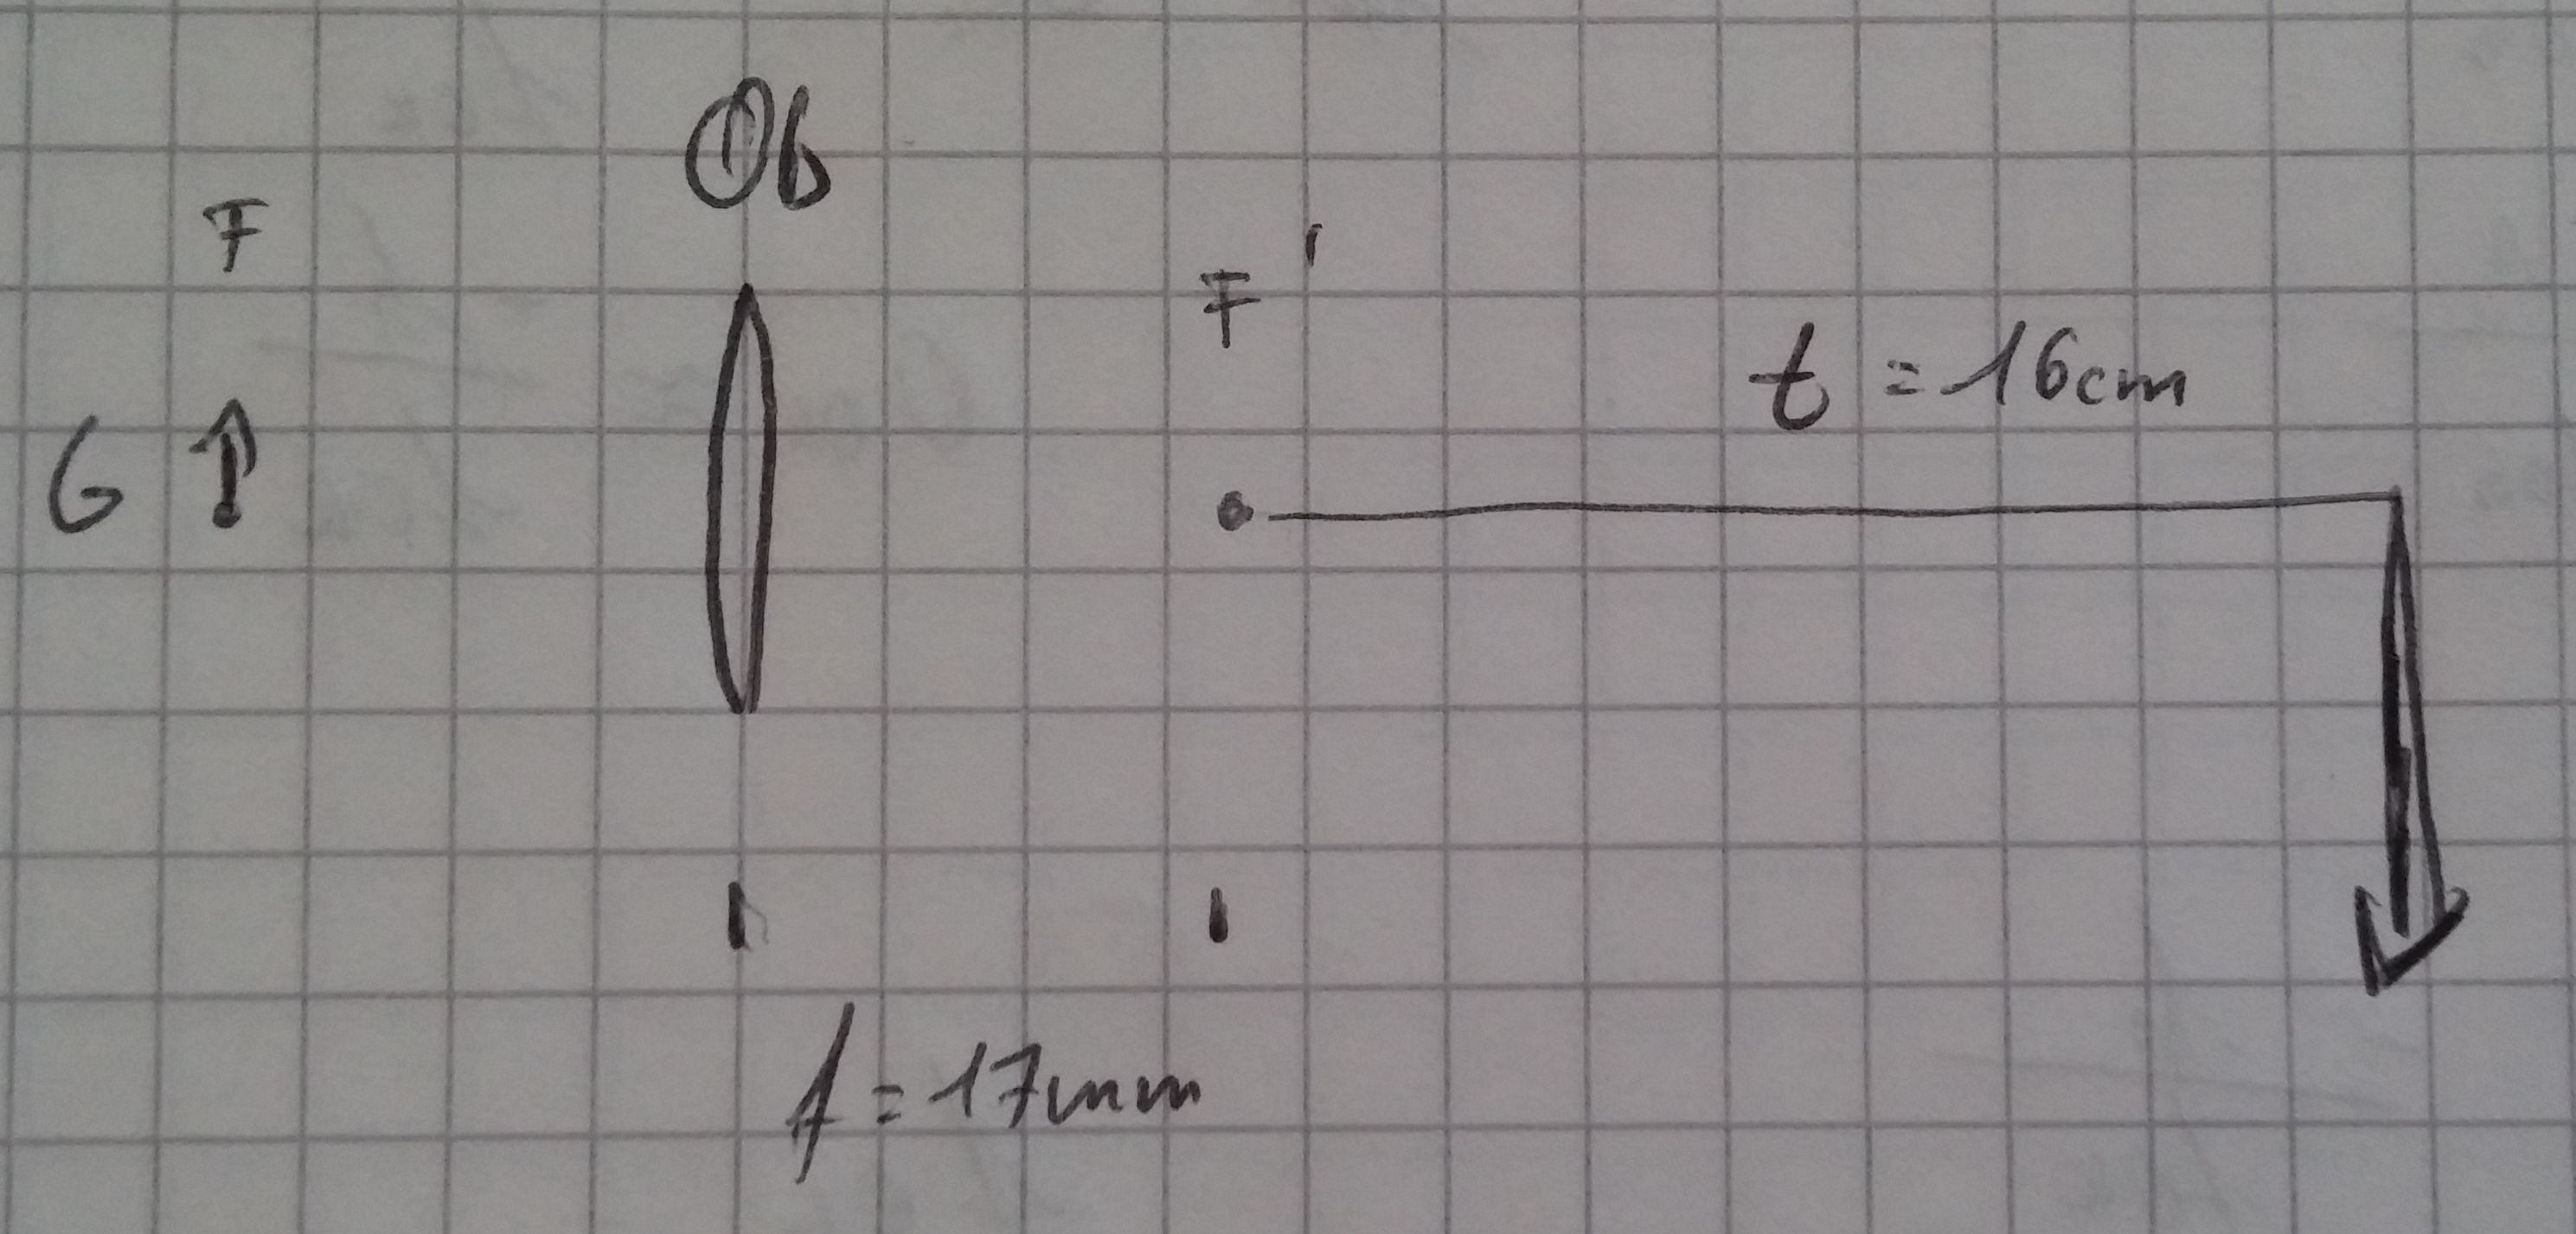
\includegraphics[scale=0.12]{A5_1.jpg}
\end{figure}

\subsection*{a)}


\begin{align*}
\frac{1}{g} &= \frac{1}{f} - \frac{1}{b} = \frac{1}{1,7} - \frac{1}{16 + 1,7} \\
\Leftrightarrow g &= \unit[1,8]{cm}
\end{align*}


\subsection*{b)}

\begin{align*}
V_M &= - \frac{t}{f_{Ob}} \cdot \frac{S_0}{f_{Ok}} = - \frac{16}{1,7} \cdot \frac{25}{3,1} = - 46,1
\end{align*}


\section{Aufgabe 6}

Die Situation ist wie auf dem Bild dargestellt:

\begin{figure}[h]
	\centering
	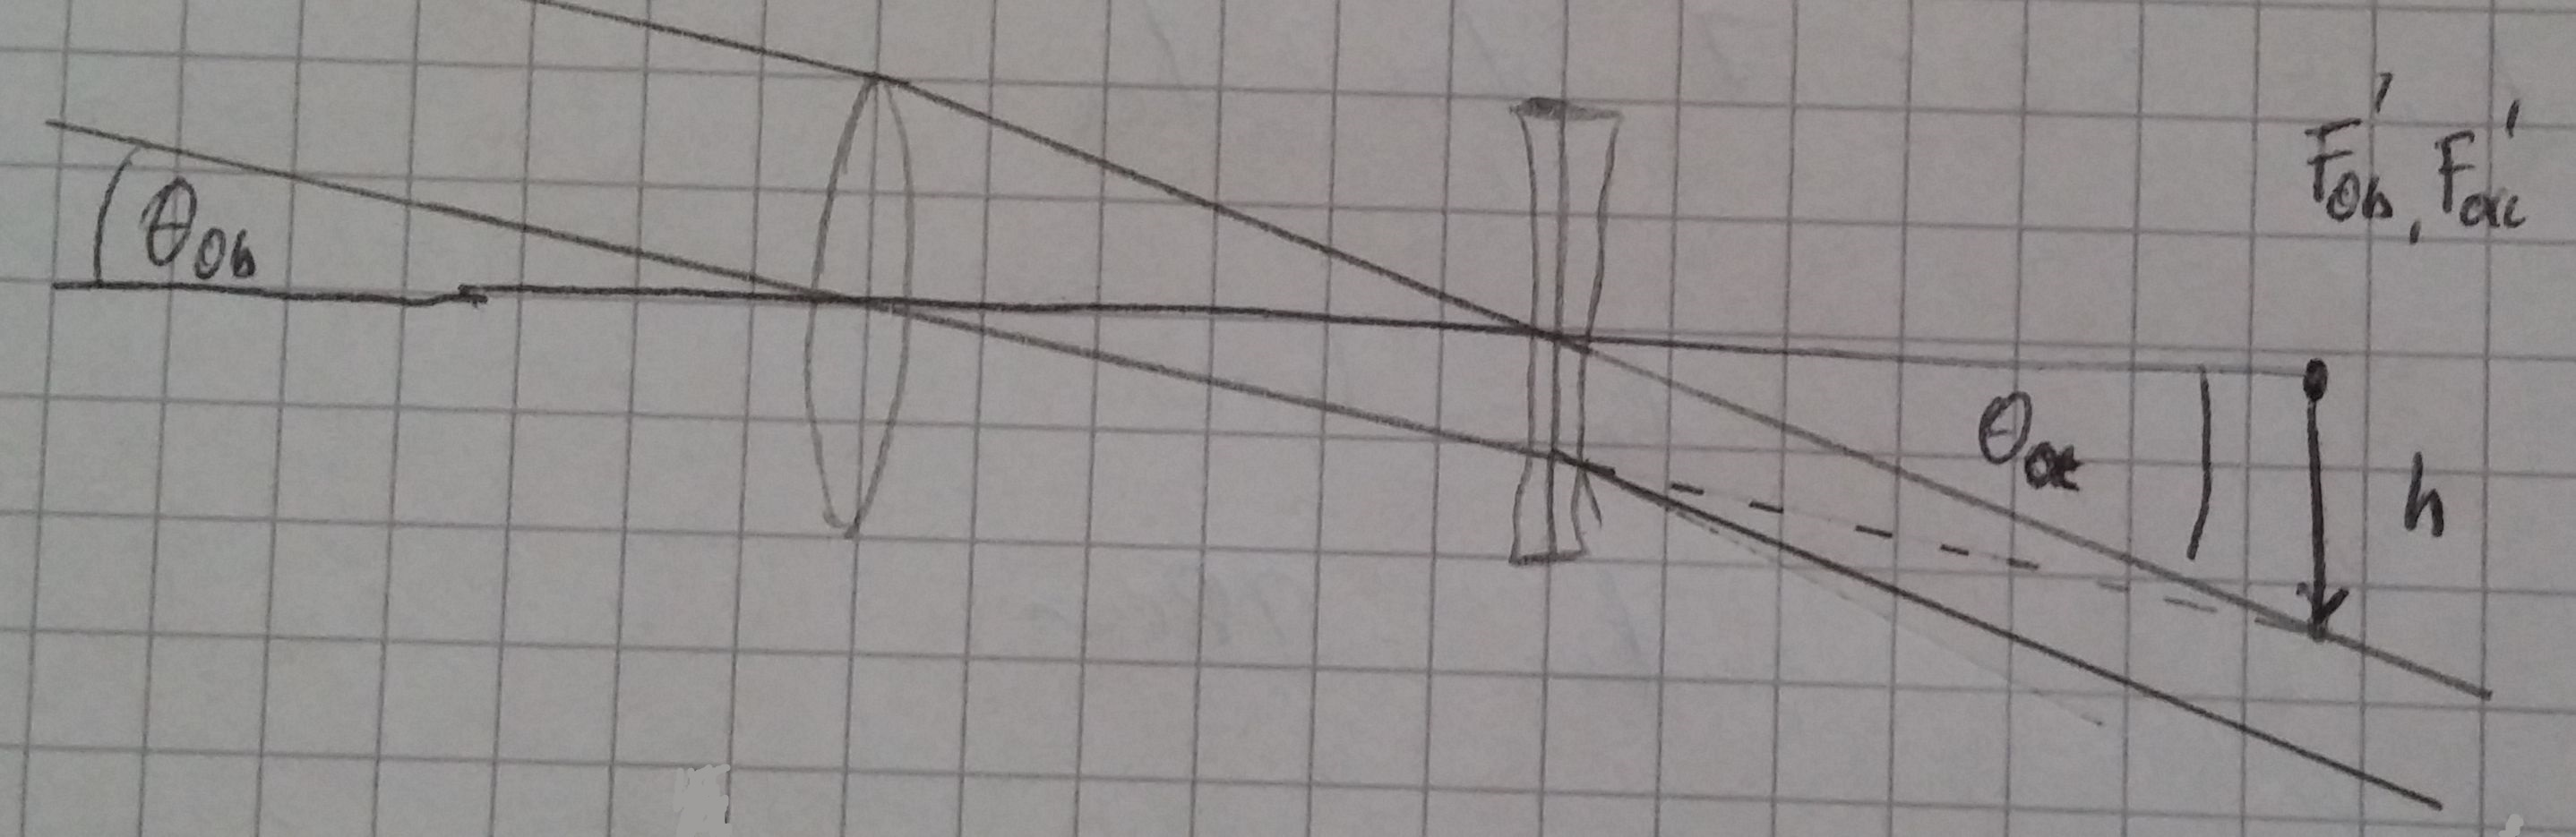
\includegraphics[scale=0.12]{A6_1.jpg}
\end{figure}

\hfill \\

Vom Teleskop wissen wir zudem das gilt $V_T = \frac{\theta_{Ok}}{\theta_{Ob}}$.

\begin{align*}
\intertext{Für das Objektiv gilt:}
\tan \left( \theta_{Ob} \right) &= \frac{h}{f_{Ob}} \\
\Rightarrow \theta_{Ob} \approx \frac{h}{f_{Ob}}
\intertext{Das gleiche giltfür das Okular:}
\tan \left( \theta_{Ok} \right) &= \frac{-h}{f_{Ok}} \\
\Rightarrow \theta_{Ok} \approx \frac{-h}{f_{Ok}}
\intertext{Die Vergrößerung ist dann:}
V_T &= \frac{ \frac{-h}{f_{Ok}}}{\frac{h}{f_{Ob}}} = - \frac{f_{Ob}}{f_{Ok}} > 0
\end{align*}

Das Bild ist damit aufrecht und virtuell.












\end{document}